\documentclass[10pt,a4paper]{article}
\usepackage[utf8]{inputenc}
\usepackage{amsmath}
\usepackage{amsfonts}
\usepackage{amssymb}
\usepackage{makeidx}
\usepackage{graphicx}
\usepackage[left=2cm,right=2cm,top=2cm,bottom=2cm]{geometry}
\author{Universidad Politécnica De La Zona Metroplitana de Guadalajara \\\\ Alumno:\\ Jiménez Cortés Raúl \\\\ Carrera:\\ Ingeniería Mecatrónica\\\\ Grupo:\\ 4ª "B" \\\\
Materia:\\ Sistemas Electrónicos De Interfaz \\\\ Profesor:\\ Morán Garabito Carlos Enrique}
\title{EV-1-6-EXPLICAR LA OPERACIÓN DE LOS CIRCUITOS DE ACTIVACIÓN CON TRISTORES EN CONVERTIDORES CA-CD Y CA-CA}
\date{24/Septiembre/2019}


\begin{document}
\begin{figure}
\centering

\includegraphics[scale=1]{Pa.jpg}
\end{figure}

\maketitle

\newpage
\section{Activación De Tristores En Convertidores CA-CD y CA-CA}
La electrónica de potencia revolucionó la capacidad de controlar grandes cantidades de
energía con eficiencia, aunado a esto, gracias a la unión que existe entre ésta disciplina
y la electrónica digital, se tienen aplicaciones a nivel educacional, industrial, etc., siendo
la más importante en ésta última, el control de máquinas eléctricas.
En un inicio las primeras máquinas eléctricas fueron accionadas por motores de CA con
velocidad constante, posteriormente, fue necesario controlar la velocidad de manera más
exacta, para lo cual se encontraron mayores ventajas en los motores de CD, debido a
que los motores de CA operan a una velocidad constante y tienden a desperdiciar una
gran cantidad de energía. Por lo tanto, debido a sus características especiales, el motor
de CD ha sido el más utilizado en la industria, donde se toma como alimentación un
sistema trifásico de CA que debe ser rectificado y posteriormente actuar como un control
de velocidad ajustable para el motor. El accionamiento de CD emplea aspectos básicos
de las técnicas de conversión de potencia, para poder controlar la velocidad y el par en
un motor de CD, considerando las diferentes cargas a las que pueda ser sometido; de
hecho, un controlador de CD debe ser capaz de modificar los diferentes niveles de voltaje
y corriente para responder de forma apropiada a cualquier cambio en la carga.
Sin embargo, para la alimentación de éste tipo de motores es necesaria una CD, la cual
no puede obtenerse directamente de una conexión eléctrica normal; para ésta
conversión, ya sea de monofásica o trifásica, es necesario un convertidor CA-CD que
realice la función de rectificación.
Aunque el objetivo de un convertidor CA-CD es transformar la tensión alterna en continua,
deben tomarse en cuenta otros aspectos para poder seleccionar y utilizar correctamente
estos circuitos, debido a que en la práctica la tensión de salida en un convertidor CA-CD
no es totalmente continua. Los convertidores CA-CD presentan diferentes topologías en
función de las características de las tensiones de entrada y salida.
Si la tensión alterna de entrada tiene una frecuencia y valor eficaz constante, y se
pretende conseguir una tensión continua de salida en todo momento, es conveniente utilizar rectificadores no controlados, sin embargo, si la salida debe ser ajustada a
diferentes valores, el rectificador debe tener algún tipo de control, por lo tanto debe usarse
un convertidor controlado.
Según su rango de potencia, los convertidores se clasifican de la siguiente forma:
\begin{figure}[hbtp]
\centering
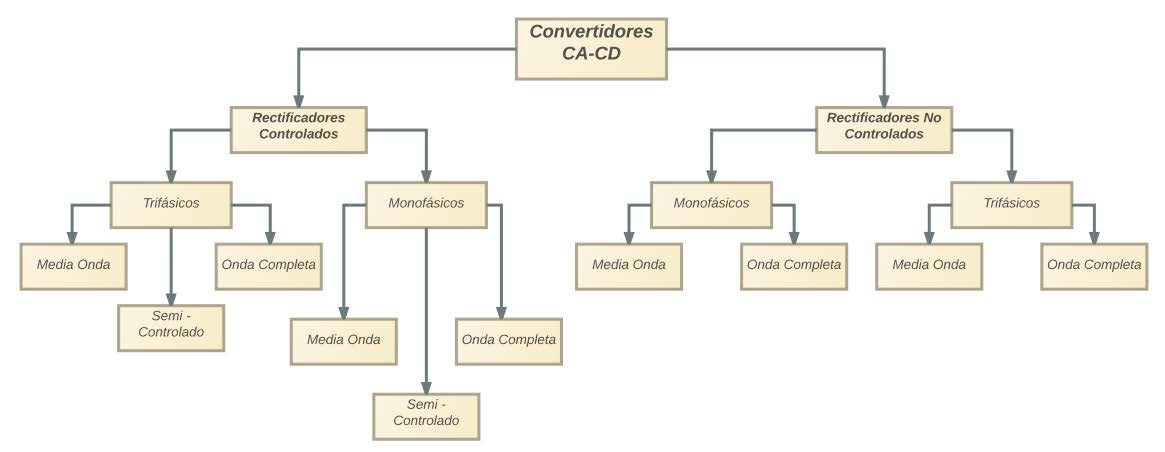
\includegraphics[scale=0.4]{diagrama.png}
\caption{Clasificación de los convertidores según el tipo de entrada, salida y potencia de
conversión.}
\end{figure}\\
Para lograr entender el funcionamiento de éstos circuitos, la simulación es de vital
importancia, debido a que la observación de manera gráfica es más fácil de comprender.
Se tiene, al realizar las simulaciones, que el comportamiento ideal es diferente al real, sin
embargo con base en las gráficas se puede obtener un panorama más exacto sobre el
funcionamiento de cada circuito y cada componente involucrado.\\
Los diodos rectificadores proporcionan sólo un voltaje de salida fijo, sin embargo, para
obtener voltajes de salida controlados, se usan tiristores con control de fase.
El voltaje de salida de los rectificadores de tiristor se varía controlando el ángulo de
retardo, por lo tanto, el tiristor se activa aplicando un pulso corto a su compuerta y se
desactiva por conmutación natural. Estos rectificadores controlados por fase son sencillos
y menos costosos, y su eficiencia es, por lo general, superior al 95%. Debido a que
convierten CA a CD, estos rectificadores controlados se le llama también convertidores
CA-CD.\\
Su misión fundamental es proporcionar energía eléctrica en forma de corriente continua
a partir de una fuente de corriente alterna.
Principalmente, se requieren de tres características para un convertidor CA-CD de
calidad:\\
1. Que produzca a su salida una tensión continua con un contenido mínimo de
armónicos.\\
2. Que no distorsione las corrientes de entrada (debe mantenerlas tan senoidales
como sea posible para no afectar a otros dispositivos conectados a la red).\\
3. Que no desfase tensión y corriente de entrada, es decir, que su factor de potencia
sea cercano a la unidad.\\\\
Los convertidores ca/ca permiten realizar, en términos generales, la conversión de corriente alterna en corriente  alterna.  En  la  práctica,  esta  transformación  se  reduce  a  una  reducción  del  valor  eficaz  de  la  tensión de entrada, y en algunos casos, a una reducción de la frecuencia de entrada que puede tomar únicamente  algunos  valores.  Desde  el  punto  de  vista  práctico,  este  tipo  de  convertidores  se  utilizan habitualmente en la construcción de arrancadores suaves para motores asíncronos, reguladores de luz, reguladores de temperatura de calderas y calentadores y otras aplicaciones industriales. A pesar de que no  se  utilizan  demasiado  en  el  mundo  de  las  telecomunicaciones,  resulta  interesante  revisar  su  estructura y características de funcionamiento. En  la  figura 2 se  muestra  el  circuito  eléctrico  básico  de  un  convertidor  ca/ca  monofásico.  Como  puede   observarse,   el   circuito   está   formado   por   dos   tiristores   conectados   en   antiparalelo.   En   aplicaciones  de  poca  potencia,  es  posible  encontrar  circuitos  donde  los  tiristores  se  sustituyen  por  triacs. Sin embargo, en aplicaciones de media y gran potencia, resulta más frecuente utilizar tiristores, ya que éstos son más robustos y fiables. \\
\begin{figure}[hbtp]
\centering
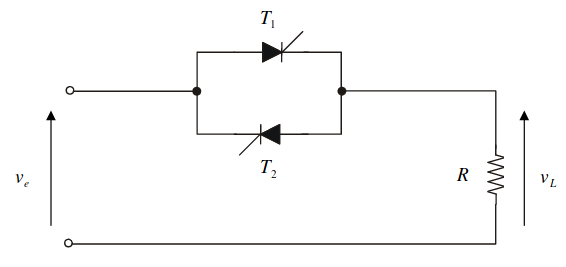
\includegraphics[scale=0.4]{Circuito.png}
\caption{Circuito básico de un convertidor ca/ca monofásico. }
\end{figure}\\
Como resulta lógico, el control de la tensión de salida se realiza mediante los ángulos de encendido de los tiristores T1 y T2. Dicho control puede ser realizado de dos formas básicas:\\-Control todo/nada. Basado en la activación y desactivaciónde la salida durante unos ciclos de forma completa. \\
-Control de fase. Basado en recortar la señal de entrada para reducir su valor eficaz.\\
-Control todo/nada\\
Este tipo de control se basa en la activación/desactivación periódica de los tiristores para conseguir que la  salida  sea  activa  durante  n  ciclos  y  esté  desconectada  durante  otros  m.  De  esta  forma,  el  efecto global que se consigue es una reducción del valor eficaz. En la figura 3 se muestra la formas de onda de salida en este tipo de control. Si el valor eficaz de la tensión de entrada al convertidor es Ve,rms, el valor eficaz de la tensión vL será:\\
\begin{figure}[hbtp]
\caption{•}
\centering
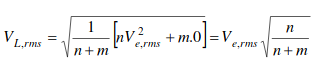
\includegraphics[scale=0.4]{ec.png}
\end{figure}\\
Si se denomina por la letra k al ciclo de trabajo:\\
\begin{figure}[hbtp]
 \caption{•}
 \centering
 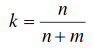
\includegraphics[scale=0.4]{ecc.png}
 \end{figure}\\
donde k puede variar entre 0 y 1. \\\begin{figure}[hbtp]
\centering
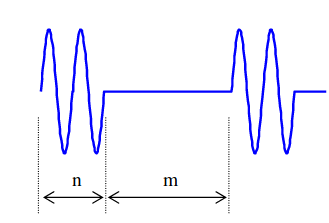
\includegraphics[scale=0.4]{ondaa.png}
\caption{Formada de onda de la tensión de salida de un convertidor ca/ca con control todo/nada. }
\end{figure}\\
Se  observa  de  esta  forma  cómo  es  posible  utilizar  este  convertidor  para  reducir  el  valor  eficaz  de  la  tensión de entrada. Este método no es aplicable, sin embargo, a cualquier tipo de aplicación. Un equipo electrónico  no  puede,  en  general,  estar  sin  alimentación  durante  m  ciclos,  ya  que  es  posible  que  los  circuitos  digitales  sufran  un  reset.  Normalmente,  este  tipo  de  control  se  utiliza  en  la  gestión  de  resistencias  de  calentamiento,  dado  que  la  inercia  térmica  del  conjunto  es  muy  superior  al  ritmo  de  variación eléctrico.\\
-Control de fase\\ El control de fase resulta similar al realizado en el caso del rectificador de media onda controlado. La diferencia radica únicamente en la topología simétrica de este tipo de convertidor. Así, en la figura 6 se  muestra  la  forma  de  onda  de  la  tensión  de  salida.  A  partir  del  ángulo  de  encendido  es  posible  controlar el valor eficaz de salida:\\
\begin{figure}[hbtp]
\caption{•}
\centering
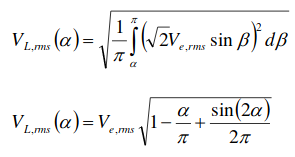
\includegraphics[scale=0.4]{ecn.png}
\end{figure}\\
Se deja como ejercicio al lector comprobar que la tensión media de salida es nula.\\
\begin{figure}[hbtp]
\centering
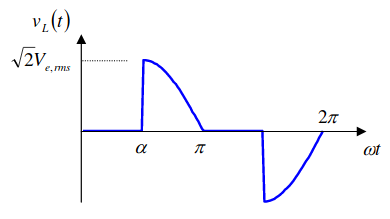
\includegraphics[scale=0.4]{onda.png}
\caption{ Forma de onda de la tensión de salida de un convertidor ca/ca con control de fase.}
\end{figure}
\\


\bibliography{EV-1-6-EXPLICAR LA OPERACIÓN DE LOS CIRCUITOS DE ACTIVACIÓN CON TRISTORES EN CONVERTIDORES CA-CD Y CA-CA.bib}{https://ocw.unican.es/pluginfile.php/1986/course/section/2310/convertidores.pdf}
\bibliographystyle{plain}
\end{document}